%!TeX root=../tese.tex
%(dica para o editor de texto: este arquivo é parte de um documento maior)
% para saber mais: https://tex.stackexchange.com/q/78101/183146

\chapter{Perceptron multi-camadas}
\label{cap:perceptron}

Neste capítulo é descrita a implementação e funcionamento de uma versão do algoritmo \eng{perceptron}, feito a partir de um núcleo básico disponibilizado no livro de Kopec \citep{classic}, e a partir do qual foram feitas modificações e criação de novos métodos de treinamento, de validação e de avaliação do treinamento.

O perceptron aqui implementado pode ser usado tanto para tarefas de classificações, quanto para tarefas de regressões de dados, e neste capítulo são apresentados exemplos de ambos os usos, embora o foco deste trabalho seja na versão de classificação.

\section{Derivação matemática do algoritmo de retropropagação}

Para a aprendizagem supervisionada foi utilizado o algoritmo de retropropagação (\eng{retropropagation}), que consiste na minimização de uma função de custos, a partir do gradiente, ou seja, da derivada desta função de custos, neste caso o erro quadrático médio, conforme foi definido no capítulo anterior.

De acordo com Kopec \citep{classic}, o perceptron consiste de uma rede cujo sinal, ou seja, os dados, se propagam em uma só direção, da camada de entrada para a camada de saída, passando pelas camadas ocultas uma a uma, e por isso o nome de rede \eng{feedforward} ao perceptron. Por sua vez, o erro que determinamos na camada final propaga-se no caminho inverso, sendo distribuídas correções da saída para a entrada, afetando aqueles neurônios que foram mais responsáveis pelo erro total. Por isso o nome de retropropagação.

Estendendo as definições já usadas no capítulo anterior, segue a derivação matemática do algoritmo de retropropagação. Como ficará claro mais à frente, podemos derivar as contas para apenas um neurônio por camada sem perda de generalidade. Dessa forma, se temos uma rede com $L$ camadas, o erro quadrático para um neurônio da camada de saída (a camada $L$) será:
\[
C_0 = (a^{(L)} - y)^2
\]
onde $y$ é a saída esperada, e $a^{(L)}$ é a saída de um neurônio da camada de saída.

Temos que $C_0$ é uma função de $a^{(L)}$, uma vez que $y$ é um valor fixo conhecido. Por sua vez, temos que de modo geral a saída de um neurônio é uma função do tipo:
\[
a^{(L)} = \sigma(w^{(L)}~a^{(L-1)} + b^{(L)})
\]
onde escrevemos $a^{(L-1)}$ é a saída do neurônio da camada anterior, $w^{(L)}$ é o \defi{peso} atribuido a essa saída, o que seria o parâmetro angular $A$ na Figura \ref{fig:neuronio}, e $b^{(L)}$ é o chamado \defi{viés} desse neurônio, análogo ao parâmetro linear de uma reta. Por fim temos a \defi{função de ativação} que escrevemos como $\sigma$ que é aplicada à essa equação linear.

Nota-se que internamente à função de ativação, um neurônio se comporta como uma transformação linear dos neurônios da camada anterior. Caso tivéssemos $n$ neurônios na camada anterior à de saída, teríamos então $n$ pesos, denotados com índice $i$ dessa forma: $\{ w_i^{(L)} \}_{i=1}^n$. Cabe assim à função de ativação, dar o comportamento não-linear à rede perceptron.

Como o objetivo é minimizar $C_0$, temos que calcular a influência dos pesos e dos viéses nesse custo. Já sabemos que isso será obtido com o gradiente, isto é, a derivada dessa função em relação a esses parâmetros que, são os únicos que podemos otimizar. De forma mais clara, temos que no início do treinamento da rede, atribuímos valores aleatórios aos pesos e aos viéses, e então executamos o \eng{feedforward}, de forma que a rede irá calcular sequencialmente os valores de saída em todas as suas camadas, obtidos a partir dos dados de entrada, que serão fixos, e desses parâmetros inicialmente aleatórios. A partir daí, poderemos otimizar esses parâmetros, exatamente da forma que estamos construindo.

O cálculo dessas derivadas é feito segundo a regra da cadeia, e adicionalmente iremos denotar a transformação linear interna à função de ativação por $z^{(L)} = w^{(L)}~a^{(L-1)} + b^{(L)}$, de forma que $a^{(L)} = \sigma(z^{(L)})$. Assim, ficamos com as derivadas para a camada de saída:

\begin{equation}\label{retro:1}
\frac{\del C_0}{\del w^{(L)}} = \frac{\del z^{(L)}}{\del w^{(L)}} \frac{\del a^{(L)}}{\del z^{(L)}} \frac{\del C_0}{\del a^{(L)}}
\end{equation}

\begin{equation}\label{retro:2}
\frac{\del C_0}{\del b^{(L)}} = \frac{\del z^{(L)}}{\del b^{(L)}} \frac{\del a^{(L)}}{\del z^{(L)}} \frac{\del C_0}{\del a^{(L)}}
\end{equation}

Para a camada de saída, podemos calcular diretamente cada termo dessas derivadas:

\begin{equation}\label{retro:4}
\frac{\del C_0}{\del a^{(L)}} = 2(a^{(L)} - y) ~\propto~ (a^{(L)} - y)
\end{equation}

\begin{equation}\label{retro:5}
\frac{\del a^{(L)}}{\del z^{(L)}} = \sigma^{'}(z^{(L)})
\end{equation}

\begin{equation}\label{retro:6}
\frac{\del z^{(L)}}{\del w^{(L)}} = a^{(L-1)}
\end{equation}

\begin{equation}\label{retro:7}
\frac{\del z^{(L)}}{\del b^{(L)}} = 1
\end{equation}

O que resulta, fazendo todas as substituições, em:

\begin{equation}\label{retro:10}
\frac{\del C_0}{\del w^{(L)}} = a^{(L-1)}~ \sigma^{'}(z^{(L)})~ (a^{(L)} - y)
\end{equation}

\begin{equation}\label{retro:11}
\frac{\del C_0}{\del b^{(L)}} = \sigma^{'}(z^{(L)})~ (a^{(L)} - y)
\end{equation}

Na equação \ref{retro:4} ocultamos o termo constante $2$ sob um símbolo de proporção, que a seguir iremos também ocultar, uma vez que usaremos o algoritmo do gradiente descendente, e assim, em seu lugar, e na verdade, todas as derivadas aqui mostradas serão multiplicadas pelo termo $\eta$, a \defi{taxa de aprendizagem}, conforme explicado no capítulo anterior. 

Analogamente, podemos pensar numa forma de fazer esses cálculos para as camadas ocultas. A princípio, podemos calcular:

\begin{equation}\label{retro:3}
\frac{\del C_0}{\del a^{(L-1)}} = \frac{\del z^{(L)}}{\del a^{(L-1)}} \frac{\del a^{(L)}}{\del z^{(L)}} \frac{\del C_0}{\del a^{(L)}}
\end{equation}

Usando o fato de que:

\begin{equation}\label{retro:8}
\frac{\del z^{(L)}}{\del a^{(L-1)}} = w^{(L)}
\end{equation}

Agora, seja a $i$-ésima camada oculta tal que $1 < i < L$, se observarmos a equação \ref{retro:3}, e fizermos $i = L-1$, usando a equação \ref{retro:8}, ficamos com:

\begin{equation}\label{retro:9}
\frac{\del C_0}{\del a^{(i)}} = w^{(i+1)} \frac{\del a^{(i+1)}}{\del z^{(i+1)}} \frac{\del C_0}{\del a^{(i+1)}}
\end{equation}

Podemos observar que há um mesmo termo duplo que aparece tanto nas equações \ref{retro:1} e \ref{retro:2} quanto na equação \ref{retro:9} acima, de forma que apenas o índice da camada é diferente. Para simplificar podemos nomear esse termo de \emph{delta da camada $i$}:

\begin{equation}\label{retro:12}
\Delta^{(i)} = \dfrac{\del a^{(i)}}{\del z^{(i)}} \dfrac{\del C_0}{\del a^{(i)}}
\end{equation}

Simplificando todas as demais expressões usando essa definição, ficamos com:

\begin{equation}\label{retro:13}
\frac{\del C_0}{\del w^{(i)}} = a^{(i-1)} \Delta^{(i)}
\end{equation}

\begin{equation}\label{retro:14}
\frac{\del C_0}{\del b^{(i)}} = \Delta^{(i)}
\end{equation}

Como vemos, as derivadas que precisamos todas dependem desse termo $\Delta$, que por sua vez depende do cálculo do termo $\dfrac{\del C_0}{\del a^{(i)}}$ que será calculado de 2 formas distintas:

\[ \dfrac{\del C_0}{\del a^{(i)}} = w^{(i+1)}~ \Delta^{(i+1)}  \;\;\Rightarrow \]
\begin{equation}\label{retro:15}
\Delta^{(i)} = \sigma^{'}(z^{(i)})~ w^{(i+1)}~ \Delta^{(i+1)}
\end{equation}
para as camadas ocultas.


\[ \dfrac{\del C_0}{\del a^{(L)}} = (y - a^{(L)}) \;\;\Rightarrow \]
\begin{equation}\label{retro:16}
\Delta^{(L)} = \sigma^{'}(z^{(L)})~ (y - a^{(L)})
\end{equation}
para a camada de saída.

Percebe-se a natureza recursiva do algoritmo, onde o caso base é calculado na camada de saída, e que o cálculo vai propagando-se para as camadas ocultas, em direção à camada de entrada. Por essa mesma razão, pudemos derivar as contas para uma camada, e no fim elas estão prontas pra serem implementadas para qualquer número de camadas ocultas. 

Outro fato útil é que a expressão interna do neurônio é uma transformação linear, assim as contas podem ser facilmente ajustadas para o caso geral em que há $n_i$ neurônios em dada camada $i$ da rede, conforme já explicado, e que será detalhado diretamente nos trechos de código que serão mostrados a seguir na implementação propriamente dita.

\section{Implementação do algoritmo de retropropagação}

A implementação seguiu uma estrutura orientada a objetos, voltemos então à representação visual da rede perceptron, a partir da imagem \ref{fig:estrutura_rn}. Cada círculo representa um neurônio, cada coluna vertical de neurônios é uma camada da rede, uma das camadas, a camada oculta nesse caso, está destacada em roxo na imagem. As setas representam as conexões entre as camadas de neurônios, cada neurônio de uma camada está ligado a todos os neurônios da camada anterior, o sentido dessa conexão é da esquerda pra direita, o que indica o processo de \eng{feedforward} da rede.

\begin{figure}[htb]
\centering
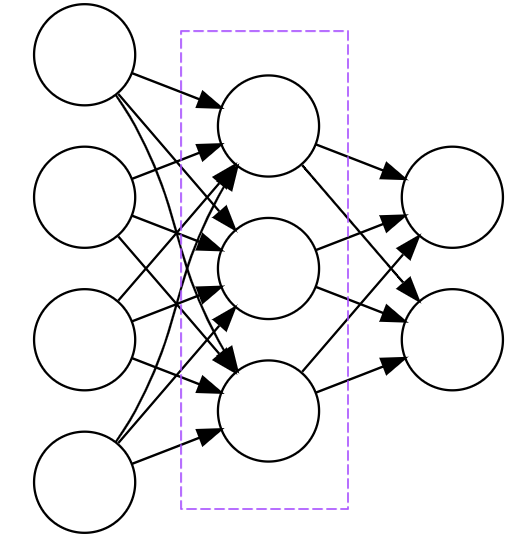
\includegraphics[width=6cm]{figuras/estrutura_rn}
\caption{Visão estrutural da rede perceptron. A linha tracejada destaca uma das camadas da rede.}
\label{fig:estrutura_rn}
\end{figure}

A implementação do perceptron deste trabalho teve como base a implementação feita por Kopec \cite{classic}, a partir da qual foram adicionados outros recursos, como o viés dos neurônios, não presentes na implementação de Kopec, como o uso da biblioteca \emph{Numpy} para o uso de seus métodos mais eficientes para lidar com listas de números de ponto flutuante. Além dessa base, também estão implementadas várias outras classes, que serão explicadas de modo mais geral.

O primeiro passo é implementar a classe \emph{Neuron} para representar cada neurônio. Esta é uma classe de entidade bem simples, contendo apenas um construtor, e o método \eng{output} que recebe os valores de entrada para esse neurônio e faz o cálculo da transformação linear e a seguir aplica e retorna o valor da função de ativação utilizada, que é passada como parâmetro ao construtor da classe. A listagem \ref{lst:neuron} abaixo mostra este método, em conjunto com o construtor da classe.

\begin{scriptsize}
\estiloR
\begin{lstlisting}[caption={Trecho da classe Neuron}, label={lst:neuron}, escapeinside={\%}]
class Neuron:
    def __init__(self, weights, bias, learning_rate, ativacao, der_ativacao):
        '''(list[float], float, float, Callable, Callable) -> None
        Construtor do Neurônio
        '''
        self.weights = weights
        self.bias = bias
        self.ativacao = ativacao
        self.der_ativacao = der_ativacao
        self.learning_rate = learning_rate
        self.output_cache = 0.0
        self.delta = 0.0

    def output(self, inputs):
        '''(list[float]) -> float
        Computa valor de ativação do neurônio, salvando o valor
        antes da função de ativação ser aplicado e retornado
        '''
        self.output_cache = np.dot(inputs, self.weights) + self.bias
        return self.ativacao(self.output_cache)
\end{lstlisting}
\end{scriptsize}

A função \emph{np.dot} da biblioteca \emph{Numpy} é utilizada para calcular o produto escalar entre os valores de entrada e os pesos desse neurônio. O valor da transformação linear é armazenado num atributo de classe antes da aplicação da função de ativação, pois será utilizado mais à frente durante o treinamento da rede.